\documentclass[11pt,a4paper]{report}
\usepackage[utf8]{inputenc}
\usepackage[T1]{fontenc}
\usepackage{geometry}
\geometry{margin=1in}
\usepackage{graphicx}
\usepackage{setspace}
\usepackage{titlesec}
\usepackage{array}
\usepackage{booktabs}
\usepackage{caption}
\usepackage{amsmath,amssymb}
\usepackage{float}
\usepackage{xcolor}
\usepackage{listings}
\usepackage{tikz}
\usetikzlibrary{shapes.geometric,arrows.meta,positioning,fit,calc}

% Section numbering depth
\setcounter{secnumdepth}{3}
\renewcommand{\thesection}{\arabic{section}}

% ---- code listings ----
\lstdefinestyle{py}{language=Python,basicstyle=\ttfamily\scriptsize,keywordstyle=\color{blue!60!black}\bfseries,
  commentstyle=\color{green!40!black}\itshape,stringstyle=\color{red!50!black},numbers=left,numberstyle=\tiny\color{gray},
  numbersep=5pt,frame=single,breaklines=true,showstringspaces=false,tabsize=4,xleftmargin=12pt,framexleftmargin=10pt}
\lstdefinestyle{term}{basicstyle=\ttfamily\scriptsize,frame=single,breaklines=true,showstringspaces=false,
  backgroundcolor=\color{gray!8},columns=fullflexible,keepspaces=true}

% ---- flowchart styles ----
\tikzset{
  fbox/.style={rectangle,draw,rounded corners=2pt,minimum height=8mm,text width=5.4cm,align=center,font=\small,fill=blue!6},
  fdec/.style={diamond,draw,aspect=2.6,align=center,font=\footnotesize,fill=yellow!18,inner sep=1pt,text width=3.4cm},
  fterm/.style={rectangle,draw,rounded corners=8pt,minimum height=7mm,align=center,font=\small\bfseries,fill=gray!18,text width=3.4cm},
  fok/.style={rectangle,draw,rounded corners=2pt,minimum height=7mm,text width=3.2cm,align=center,font=\small,fill=green!12},
  fbad/.style={rectangle,draw,rounded corners=2pt,minimum height=7mm,text width=3.2cm,align=center,font=\small,fill=red!10},
  arr/.style={-{Stealth[length=2.2mm]},thick}
}

\providecommand{\phantomsection}{}
\begin{document}

% ------------------ Cover Page ------------------
\begin{titlepage}
    \centering
    
\includegraphics[width=5cm]{College Logo RGB.jpg}\\[1cm]

    \vspace{1cm}
    \textbf{\large A Complex Engineering Problem Report on} \\[0.5cm]
    {\LARGE \textbf{Deadlock Avoidance Using the Banker's Algorithm}}\\[1.5cm]

    {\Large A9510 - Operating System Laboratory}\\[1.5cm]

    \textbf{Submitted by}\\ [0.25cm]
    Batch No. 1

    \begin{center}
        \begin{table}[h!]
            \centering
            \setstretch{1.2}
            \begin{tabular}{l l}
                {Ermala Bhanu Teja} & {25881A05S8}\\ [2mm]
                {Lingala Madhu Goud} & {25881A05U1}\\ [2mm]
                {Kasarla Harsha Vardhan} & {25881A05T6}\\ [2mm]
            \end{tabular}
        \end{table}
    \end{center}

    \vspace{0.5cm}
    \textbf{Course Facilitator}\\ [0.1in]
    {Ms. A. Ashwini}\\
    Assistant Professor\\[2.5cm]

    {\large\textbf{Department of Computer Science and Engineering}}\\[0.5cm]
    {\large\textbf{Vardhaman College of Engineering, Hyderabad}}\\[0.5cm]
    {\large \textbf{October 2026}}
\end{titlepage}

% ------------------ Contents ------------------
\tableofcontents
\newpage

% =============================================================================
\section{Introduction}
% =============================================================================

\subsection{Background}
A modern operating system runs many processes at the same time, and these processes compete for a limited number of resources such as memory buffers, files, printers, database locks and network connections. A process asks for a resource; if the resource is not free, the process waits. A \emph{deadlock} appears when every process in a set is waiting for a resource that is held by another process of the same set, so none of them can ever continue [1]. Figure~\ref{fig:rag} shows the smallest example: process $P_1$ holds resource $R_1$ and asks for $R_2$, while $P_2$ holds $R_2$ and asks for $R_1$.

\begin{figure}[h!]
\centering
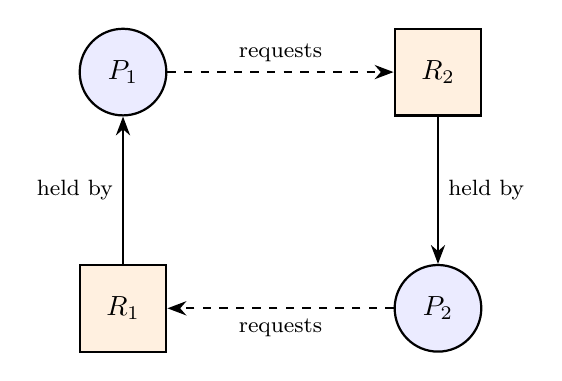
\begin{tikzpicture}[>={Stealth[length=2.4mm]},
   proc/.style={circle,draw,thick,minimum size=11mm,fill=blue!8},
   res/.style={rectangle,draw,thick,minimum size=11mm,fill=orange!12}]
  \node[proc] (p1) at (0,0) {$P_1$};
  \node[res]  (r2) at (4,0) {$R_2$};
  \node[proc] (p2) at (4,-3) {$P_2$};
  \node[res]  (r1) at (0,-3) {$R_1$};
  \draw[->,thick] (r1) -- node[left,font=\footnotesize]{held by} (p1);
  \draw[->,thick,dashed] (p1) -- node[above,font=\footnotesize]{requests} (r2);
  \draw[->,thick] (r2) -- node[right,font=\footnotesize]{held by} (p2);
  \draw[->,thick,dashed] (p2) -- node[below,font=\footnotesize]{requests} (r1);
\end{tikzpicture}
\caption{Resource-allocation graph of a deadlock: a circular wait between two processes (solid arrow = held, dashed arrow = requested).}
\label{fig:rag}
\end{figure}

Operating-system designers have three families of answers: \emph{prevent} deadlocks by making one of the necessary conditions impossible, \emph{avoid} them by granting a request only if the system stays in a safe state, or \emph{detect} them after they occur and recover [1],[2]. This report studies the second family. The classical avoidance method is the \textbf{Banker's algorithm}, proposed by Dijkstra for one resource type [4] and extended to several resource types by Habermann [5]. The operating system behaves like a careful banker: it grants a loan (a resource request) only if, after granting it, the bank could still satisfy every customer's maximum credit line in some order.

\subsection{Problem Summary}
Table~\ref{tab:summary} summarises the assigned problem.

\begin{table}[h!]
\centering
\caption{Summary of the assigned complex engineering problem.}
\label{tab:summary}
\small
\renewcommand{\arraystretch}{1.25}
\begin{tabular}{|>{\bfseries}p{3.6cm}|p{11.2cm}|}
\hline
Course component & Operating Systems -- Assignment (A9510 Operating System Laboratory) \\ \hline
Team (Batch 1) & Ermala Bhanu Teja (25881A05S8), Lingala Madhu Goud (25881A05U1), Kasarla Harsha Vardhan (25881A05T6) \\ \hline
Title & Deadlock Avoidance Using the Banker's Algorithm \\ \hline
Sustainable Development Goals & SDG 9 (Industry, Innovation and Infrastructure), SDG 16 (Peace, Justice and Strong Institutions) \\ \hline
Sustainability aspect & Safe resource utilization \\ \hline
Learning approach & Problem-Based Learning \\ \hline
Problem statement & Analyze resource-allocation and maximum-claim data to determine safe states and decide whether resource requests can be granted. \\ \hline
Duration & 2 weeks \\ \hline
Expected outcome & Apply deadlock-avoidance methods to resource allocation. \\ \hline
\end{tabular}
\end{table}

\subsection{Objectives}
\begin{itemize}
    \item To model a multi-process, multi-resource system with the data structures \emph{Available}, \emph{Max}, \emph{Allocation} and \emph{Need}.
    \item To implement the safety algorithm, which decides whether a state is safe and returns a safe sequence.
    \item To implement the resource-request algorithm, which decides whether a request is granted, made to wait, or denied because it would lead to an unsafe state.
    \item To prove and to test that the system never enters a deadlock when every grant is checked.
    \item To compare the Banker's algorithm with an unprotected system and with a deadlock-prevention policy on thousands of random workloads, and to measure the cost of the safety check.
    \item To discuss the sustainability and societal value of safe resource utilization (SDG 9 and SDG 16).
\end{itemize}

% =============================================================================
\section{Problem Definition}
% =============================================================================
\subsection{Problem Statement}
A system has $m$ resource types, each with a fixed number of identical instances, and $n$ processes. Every process declares in advance the maximum number of instances of each type that it may ever need (its \emph{maximum claim}) and then requests and releases instances one request at a time. The operating system must \textbf{decide, for every request, whether granting it immediately is safe}. A request must be refused or delayed if granting it could leave the system in a state from which a deadlock can no longer be excluded. The decision must be correct (no deadlock is ever possible after a grant), must be explainable to the user, and must be cheap enough to be executed at every request.

The main challenges are:
\begin{itemize}
    \item \textbf{Defining safety precisely.} A state is not unsafe only when a deadlock has already occurred; it is unsafe whenever no order of completion exists in which all processes can obtain their maximum claim. An unsafe state \emph{may} lead to deadlock, a safe state \emph{cannot}.
    \item \textbf{Deciding with incomplete information.} Only the maximum claims are known, not the actual order of future requests, so the decision must be valid for \emph{every} possible future behaviour of the processes.
    \item \textbf{Balancing safety and utilization.} Refusing every risky request prevents deadlock but may leave resources idle and make processes wait unnecessarily.
    \item \textbf{Keeping the decision cost low.} The safety test runs at every request and must scale with the number of processes.
    \item \textbf{Handling invalid input.} Requests larger than the declared claim, claims larger than the installed resources, and unknown processes must be detected and reported.
\end{itemize}

\subsection{Constraints and Assumptions}
\begin{itemize}
    \item The number of processes $n$ and resource types $m$ is fixed during a run; the total number of instances of every type is known and constant.
    \item Every process declares its maximum claim in advance and never asks for more than this claim ($\text{Max}_i \le \text{Total}$).
    \item A process that has received all its resources will finish in a finite time and then return everything it holds.
    \item Resources are reusable, non-preemptable and identical within one type (e.g.\ 3 printers, 7 buffers).
    \item Requests are handled one at a time and in the order in which they reach the system (no concurrent calls to the algorithm).
\end{itemize}

\subsection{Stakeholders}
\begin{itemize}
    \item \textbf{Operating-system and runtime developers}, who must integrate a resource-allocation policy into schedulers, lock managers and resource managers.
    \item \textbf{Application developers}, whose programs freeze if they take part in a deadlock.
    \item \textbf{System administrators and cloud operators}, who must keep shared servers responsive and avoid manual restarts.
    \item \textbf{End users and institutions} that rely on digital services (e.g.\ banking, e-governance, healthcare portals) and are affected by service freezes.
    \item \textbf{Students and teachers}, who need a transparent tool for learning how safe states and safe sequences work.
\end{itemize}

\subsection{Expected Outcomes}
\begin{itemize}
    \item A working Banker's-algorithm simulator that reads a system state from a file, prints a safe sequence (or reports that none exists) and processes resource requests and releases.
    \item A correctness argument and test evidence that granting only safe requests keeps the system deadlock-free.
    \item Quantitative results on deadlock probability, waiting and completion time for avoidance versus no avoidance versus prevention.
    \item A measurement of the running time of the safety algorithm as the number of processes grows.
\end{itemize}

% =============================================================================
\section{Justification as a Complex Engineering Problem}
% =============================================================================
Deadlock handling has no single algorithmic answer. Every approach gives up something (concurrency, information, run-time cost, or generality), and the best choice depends on the workload. The following solution pathways were considered.

\begin{enumerate}
    \item \textbf{Deadlock prevention}: make one of the four necessary conditions (mutual exclusion, hold and wait, no preemption, circular wait) impossible, for example by requesting all resources at once or by numbering resource types and always requesting them in increasing order [7]. It is simple and safe but lowers resource utilization.
    \item \textbf{Deadlock avoidance (Banker's algorithm)}: allow all four conditions, but grant a request only if the resulting state is safe [4],[5]. It uses resources well but needs the maximum claims in advance and runs a safety test at every request.
    \item \textbf{Deadlock detection and recovery}: grant requests freely, periodically search for a cycle (or use a matrix-based detection algorithm) and then terminate or roll back processes [6],[8]. It needs no advance information but wastes the work of the victims.
    \item \textbf{Ignoring the problem} (the ``ostrich'' approach): used by most general-purpose operating systems, which leave deadlock-free design to programmers [1]. It has zero overhead but gives no guarantee.
    \item \textbf{Protocol-based avoidance in special domains}: for example resource-ordering lock hierarchies and the priority-ceiling protocol in real-time systems [10].
\end{enumerate}

The assigned project follows pathway 2 and compares it with pathways 1 and 4 on the same workloads. The topic is a \emph{complex engineering problem} because it shows the following attributes.

\subsection{Depth of Knowledge Required}
The solution needs knowledge from several areas: operating-system concepts (processes, resources, synchronisation, the four necessary conditions of deadlock), discrete mathematics (vectors and partial orders, induction, proofs of invariants), algorithm analysis (worst-case complexity of the safety test), probability and statistics (design of random experiments and interpretation of rates over many trials), and software engineering (data validation, modular design, unit testing and reproducible experiments). The proofs in Section~\ref{sec:method} use ideas from state-space reasoning, which goes beyond routine textbook calculation.

\subsection{Conflicting Constraints and Trade-offs}
Several requirements pull against each other:
\begin{itemize}
    \item \textbf{Safety versus utilization:} the algorithm is deliberately conservative. It may delay a request that would never have caused a deadlock, because it must be correct for every possible future behaviour.
    \item \textbf{Safety versus overhead:} the safety test costs $O(mn^2)$ per request, so more safety checking means more processor time.
    \item \textbf{Generality versus information:} avoidance needs maximum claims in advance, which many real programs cannot state; prevention and detection do not need them.
    \item \textbf{Deadlock freedom versus fairness:} granting only safe requests removes deadlock but does not guarantee that a particular process is not postponed repeatedly (starvation).
\end{itemize}

\subsection{Depth of Analysis Required}
The correctness of the method cannot be taken from a formula; it has to be argued. The report (i) defines a safe state formally, (ii) proves that safe states are never deadlocked and that a checked grant keeps the system safe, (iii) proves that a process at the head of a safe sequence can always be served, (iv) checks the implementation against an exhaustive search over all execution orders on 20{,}000 random states, and (v) analyses performance experimentally because the effect of conservative denial on completion time cannot be derived in closed form.

\subsection{Familiarity of Issues}
Practical issues that engineers meet with this approach are: the maximum claim of a program is often unknown or overestimated, the number of processes changes while the system runs, resources can fail or be removed, and the safety test is repeated at every request. Many students are familiar with the textbook example, but they usually do not see why a state that is merely \emph{unsafe} is not yet a deadlock, or how a denied request is rolled back without changing the state. These points are made explicit in the design and tests of this project.

\subsection{Extent of Applicable Codes}
No law or mandatory standard prescribes the Banker's algorithm. The relevant normative guidance is indirect: POSIX (IEEE Std 1003.1) defines the behaviour of threads and mutexes that real programs use and in which deadlocks can occur [11], and ISO/IEC 25010 lists reliability (maturity, availability, fault tolerance and recoverability) as a product-quality characteristic that a deadlock-free resource manager supports [12]. The project therefore relies mainly on the classical algorithm and on good engineering practice (input validation, documented behaviour, repeatable tests) rather than on a code of practice.

\subsection{Involvement of Interested Parties}
The interested parties are those listed in Section 2.3. Their needs differ: kernel developers want a small, predictable overhead; application developers want requests to be granted quickly; operators want no frozen services; users want reliable systems; and teachers want an algorithm that is transparent. The simulator therefore prints the reason for every decision (error, wait, or unsafe) so that each party can understand and audit it.

\subsection{Interdependence of Sub-Problems}
The sub-problems cannot be solved in isolation. The \emph{safety test} is the core of the \emph{request handler}; the request handler relies on correct \emph{data validation} of claims and allocations; the quality of the decisions depends on the \emph{declared claims} (a large claim makes the algorithm more conservative); and the \emph{experimental evaluation} depends on a workload model that must be consistent with the algorithm's assumptions. A change in one part (for example, allowing a process to declare a larger claim) changes the results of all the others.

% =============================================================================
\section{Literature Review}
% =============================================================================
The deadlock problem was identified in the early multiprogramming systems of the 1960s. Dijkstra introduced the banker's idea for a single resource type in his work on cooperating sequential processes [4], and Habermann generalised it to several resource types and gave the safe-state formulation that is taught today [5]. Havender, working on the IBM OS/360 system, proposed the prevention schemes based on requesting all resources at once and on ordering resource types [7].

Coffman, Elphick and Shoshani collected the four necessary conditions for deadlock (mutual exclusion, hold and wait, no preemption and circular wait) and surveyed prevention, avoidance and detection in a single framework [6]. They observed that practical systems usually combine several techniques instead of using only one. Holt formalised deadlock with graph models and described how to detect it in systems with several resource instances [8]. These papers established the vocabulary used in all later textbooks [1]--[3].

The cost of the Banker's algorithm has been studied explicitly. Habermann's analysis shows that one execution is proportional to the square of the number of processes, and Belik presented a modified algorithm whose amortised running time is $O(mn)$ under favourable conditions, compared with $\Theta(mn^2)$ for the original [9]. This is the main practical criticism of avoidance: the test must be repeated at every request.

Textbooks note that avoidance is rarely built into general-purpose operating systems, because it needs maximum claims that programs cannot usually supply, and that deadlock-free design is mostly left to programmers [1]. In contrast, real systems use \emph{prevention-style} rules (for example, lock ordering enforced by debugging tools) and \emph{detection-style} tools. In real-time systems, protocols such as priority ceiling avoid deadlock on locks by restricting when a lock may be acquired [10]. The Banker's algorithm remains important as the reference method for explaining safe states, and it is still used where all resource requirements are known in advance, such as the allocation of a fixed pool of buffers or devices to a known set of jobs.

\textbf{Gap addressed in this project.} The cited sources describe the algorithm and its complexity, but a student cannot easily see the effect of avoidance on a whole workload. This project provides (i) an executable and transparent implementation, (ii) a machine-checked comparison of its safety decision with an exhaustive search, and (iii) a reproducible experiment that compares avoidance with no avoidance and with prevention.

% =============================================================================
\section{Methodology, Design and Engineering Analysis}
\label{sec:method}
% =============================================================================
\subsection{System Model and Notation}
The system has $n$ processes $P_0,\dots,P_{n-1}$ and $m$ resource types. The following data structures are kept (all vectors have length $m$):

\begin{table}[h!]
\centering
\caption{Data structures of the Banker's algorithm.}
\renewcommand{\arraystretch}{1.25}
\begin{tabular}{|l|p{11cm}|}
\hline
\textbf{Symbol} & \textbf{Meaning} \\ \hline
$\text{Total}[j]$ & Number of installed instances of resource type $j$. \\ \hline
$\text{Max}[i][j]$ & Maximum number of instances of type $j$ that $P_i$ may ever need (declared in advance). \\ \hline
$\text{Alloc}[i][j]$ & Instances of type $j$ currently held by $P_i$. \\ \hline
$\text{Need}[i][j]$ & Instances of type $j$ that $P_i$ may still request. \\ \hline
$\text{Available}[j]$ & Instances of type $j$ that are free now. \\ \hline
\end{tabular}
\end{table}

The derived quantities are
\begin{align}
\text{Need}[i][j] &= \text{Max}[i][j] - \text{Alloc}[i][j], \label{eq:need}\\
\text{Available}[j] &= \text{Total}[j] - \sum_{i=0}^{n-1} \text{Alloc}[i][j]. \label{eq:avail}
\end{align}
A state is \emph{valid} if $0 \le \text{Alloc}_i \le \text{Max}_i \le \text{Total}$ for every process and $\text{Available} \ge 0$; the implementation checks this when the state is loaded. For two vectors, $X \le Y$ means $X[j] \le Y[j]$ for all $j$.

\subsection{Safe State}
\textbf{Definition.} A state is \emph{safe} if there is an ordering $\langle P_{\pi(1)},\dots,P_{\pi(n)}\rangle$ of all processes, called a \emph{safe sequence}, such that for every $k$
\begin{equation}
\text{Need}_{\pi(k)} \;\le\; \text{Available} + \sum_{l<k} \text{Alloc}_{\pi(l)}. \label{eq:safe}
\end{equation}
In words: if the processes finish one after another in this order, each one finds enough free instances for its remaining need, because all earlier processes have returned what they held. A state that is not safe is \emph{unsafe}. An unsafe state is not necessarily a deadlock, but it is a state in which deadlock can no longer be excluded.

\subsection{Safety Algorithm}
The safety algorithm tests Eq.~(\ref{eq:safe}) by simulating the completion of processes (Figure~\ref{fig:safetyflow}).

\begin{enumerate}
    \item Let $\text{Work} = \text{Available}$ and $\text{Finish}[i]=\text{false}$ for every active process.
    \item Find a process $P_i$ with $\text{Finish}[i]=\text{false}$ and $\text{Need}_i \le \text{Work}$. If none exists, go to step 4.
    \item Set $\text{Work} = \text{Work} + \text{Alloc}_i$, $\text{Finish}[i]=\text{true}$, append $P_i$ to the sequence, and go to step 2.
    \item If $\text{Finish}[i]=\text{true}$ for all $i$, the state is \textbf{safe} and the sequence is a safe sequence; otherwise it is \textbf{unsafe}.
\end{enumerate}

\begin{figure}[h!]
\centering
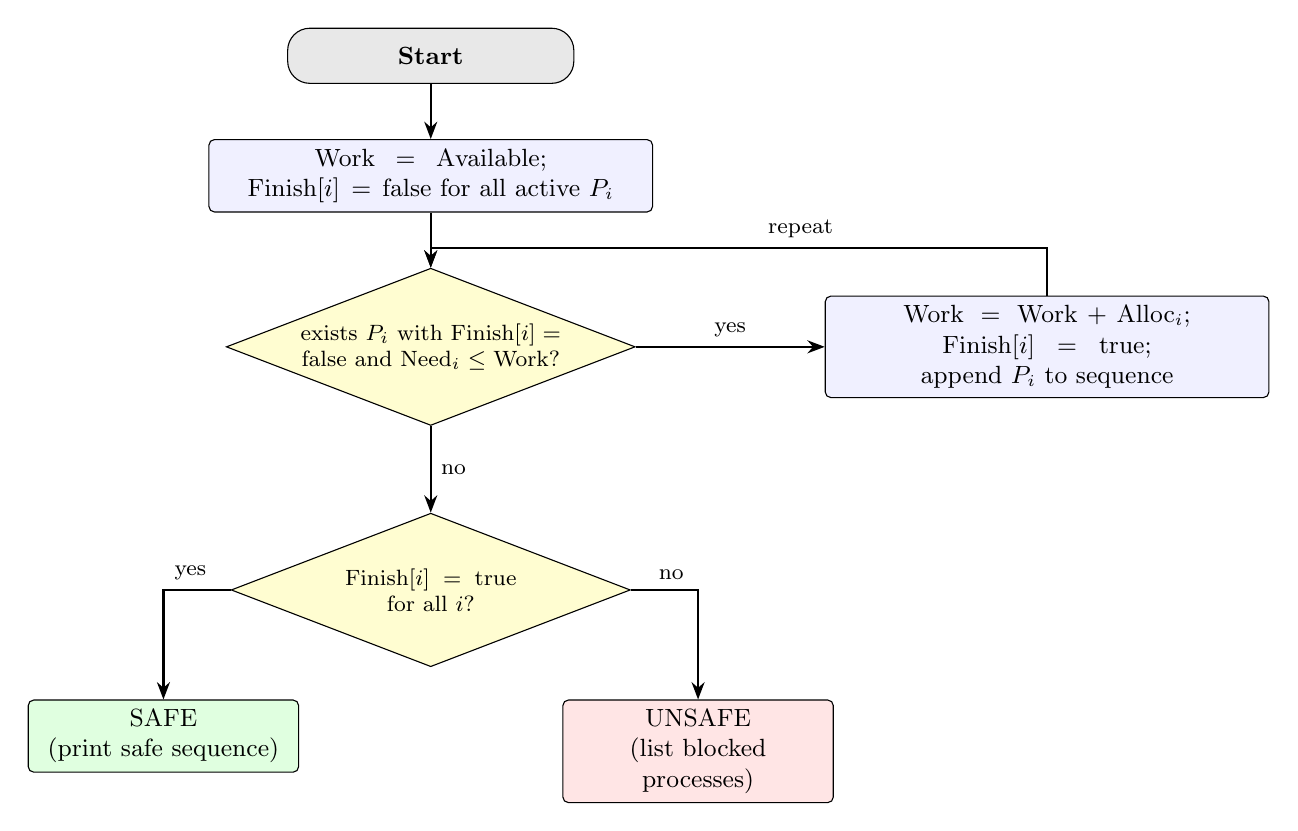
\begin{tikzpicture}[node distance=7mm]
  \node[fterm] (s) {Start};
  \node[fbox,below=of s] (a) {$\text{Work}=\text{Available}$;\\ $\text{Finish}[i]=\text{false}$ for all active $P_i$};
  \node[fdec,below=of a] (d1) {exists $P_i$ with $\text{Finish}[i]=\text{false}$ and $\text{Need}_i\le\text{Work}$?};
  \node[fbox,right=24mm of d1] (b) {$\text{Work}=\text{Work}+\text{Alloc}_i$;\\ $\text{Finish}[i]=\text{true}$;\\ append $P_i$ to sequence};
  \node[fdec,below=11mm of d1] (d2) {$\text{Finish}[i]=\text{true}$\\ for all $i$?};
  \node[fok,below left=9mm and 4mm of d2] (ok) {SAFE\\ (print safe sequence)};
  \node[fbad,below right=9mm and 4mm of d2] (bad) {UNSAFE\\ (list blocked processes)};
  \draw[arr] (s)--(a); \draw[arr] (a)--(d1);
  \draw[arr] (d1)--node[above,font=\footnotesize]{yes}(b);
  \draw[arr] (b.north) -- ++(0,6mm) -| node[pos=0.2,above,font=\footnotesize]{repeat}($(d1.north)+(0,3mm)$) -- (d1.north);
  \draw[arr] (d1)--node[right,font=\footnotesize]{no}(d2);
  \draw[arr] (d2)-|node[pos=0.3,above,font=\footnotesize]{yes}(ok);
  \draw[arr] (d2)-|node[pos=0.3,above,font=\footnotesize]{no}(bad);
\end{tikzpicture}
\caption{Flowchart of the safety algorithm.}
\label{fig:safetyflow}
\end{figure}

\subsection{Resource-Request Algorithm}
When $P_i$ makes a request $\text{Request}_i$, the following steps are executed (Figure~\ref{fig:requestflow}).
\begin{enumerate}
    \item If $\text{Request}_i \not\le \text{Need}_i$, report an error: the process has exceeded its maximum claim.
    \item If $\text{Request}_i \not\le \text{Available}$, the resources are not free: $P_i$ must wait.
    \item Otherwise \emph{pretend} to allocate: $\text{Available} \mathrel{-}= \text{Request}_i$, $\text{Alloc}_i \mathrel{+}= \text{Request}_i$, $\text{Need}_i \mathrel{-}= \text{Request}_i$, and run the safety algorithm on the new state.
    \item If the new state is safe, the allocation is \textbf{committed}. If not, the old state is restored and $P_i$ must wait: the request is denied \emph{although the resources are free}.
\end{enumerate}

\begin{figure}[h!]
\centering
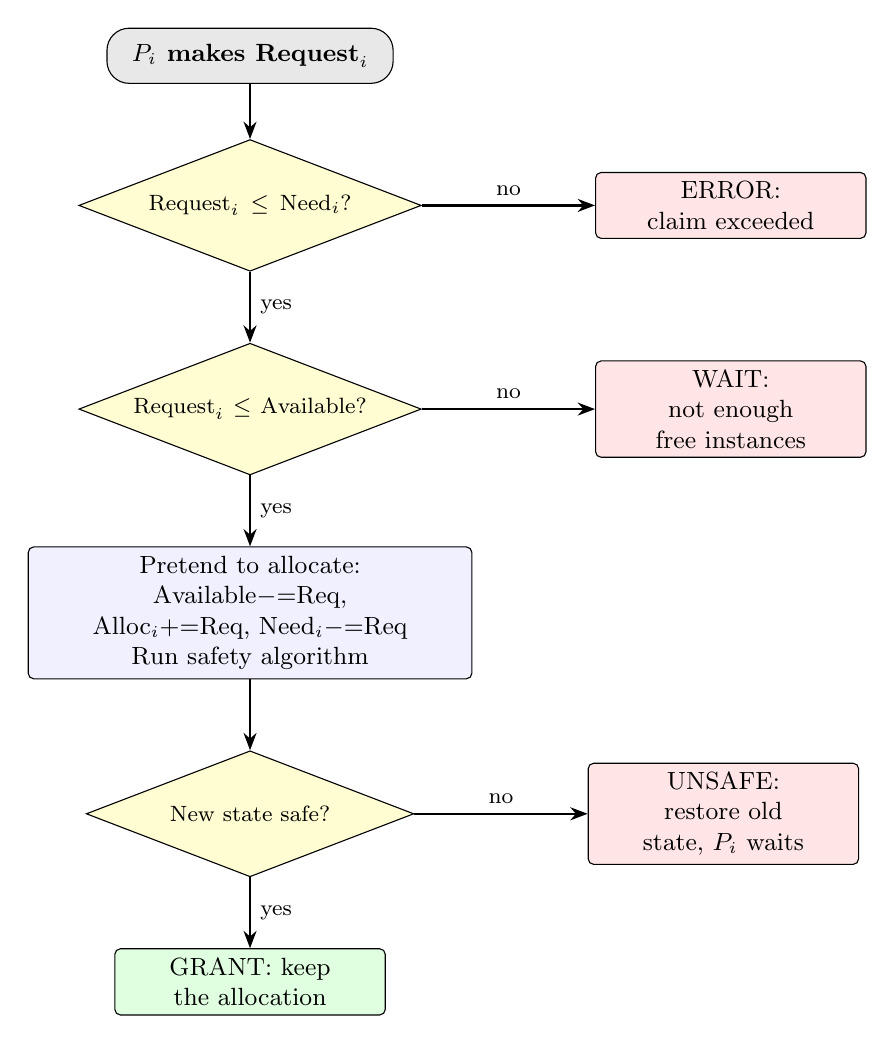
\begin{tikzpicture}[node distance=7mm]
  \node[fterm] (s) {$P_i$ makes $\text{Request}_i$};
  \node[fdec,below=of s] (d1) {$\text{Request}_i\le\text{Need}_i$?};
  \node[fbad,right=22mm of d1] (e1) {ERROR:\\ claim exceeded};
  \node[fdec,below=9mm of d1] (d2) {$\text{Request}_i\le\text{Available}$?};
  \node[fbad,right=22mm of d2] (e2) {WAIT:\\ not enough free instances};
  \node[fbox,below=9mm of d2] (p) {Pretend to allocate:\\ Available$-$=Req, Alloc$_i$+=Req, Need$_i$$-$=Req\\ Run safety algorithm};
  \node[fdec,below=9mm of p] (d3) {New state safe?};
  \node[fbad,right=22mm of d3] (e3) {UNSAFE:\\ restore old state, $P_i$ waits};
  \node[fok,below=9mm of d3] (g) {GRANT: keep the allocation};
  \draw[arr] (s)--(d1);
  \draw[arr] (d1)--node[above,font=\footnotesize]{no}(e1);
  \draw[arr] (d1)--node[right,font=\footnotesize]{yes}(d2);
  \draw[arr] (d2)--node[above,font=\footnotesize]{no}(e2);
  \draw[arr] (d2)--node[right,font=\footnotesize]{yes}(p);
  \draw[arr] (p)--(d3);
  \draw[arr] (d3)--node[above,font=\footnotesize]{no}(e3);
  \draw[arr] (d3)--node[right,font=\footnotesize]{yes}(g);
\end{tikzpicture}
\caption{Flowchart of the resource-request algorithm.}
\label{fig:requestflow}
\end{figure}

\subsection{Correctness Analysis}
\textbf{Lemma 1 (a safe state is not deadlocked).} If a state is safe with safe sequence $\langle P_{\pi(1)},\dots\rangle$, then $P_{\pi(1)}$ satisfies $\text{Need}_{\pi(1)}\le\text{Available}$, so it can obtain everything it may still need, finish and release $\text{Alloc}_{\pi(1)}$. By Eq.~(\ref{eq:safe}) the same argument applies to $P_{\pi(2)}$ with the enlarged free pool, and by induction every process can finish. Hence at least one process can always make progress.

\textbf{Lemma 2 (a checked grant keeps the state safe).} The request algorithm commits an allocation only if the safety algorithm has found a safe sequence in the new state. Therefore, if the initial state is safe, every state reached by committed grants and by process terminations is safe. A termination only adds the released instances to $\text{Available}$, so the old safe sequence without the finished process remains valid.

\textbf{Theorem (deadlock freedom).} If the system starts in a safe state and every allocation is made through the request algorithm, no deadlock can occur. \emph{Proof:} by Lemma 2 the system is always in a safe state, and by Lemma 1 a safe state always contains a process that can complete. $\square$

\textbf{Lemma 3 (progress of the head of the sequence).} Let $P_f$ be the first process of a safe sequence and let it request $r\le\text{Need}_f$. Since $\text{Need}_f\le\text{Available}$, the request is available. After the grant, $\text{Need}'_f=\text{Need}_f-r$ and $\text{Available}'=\text{Available}-r$, so $\text{Need}'_f\le\text{Available}'$ still holds, and after $P_f$ finishes the free pool is the same as before the grant. The remaining part of the sequence is unchanged, so the new state is safe and the request is granted. Hence, in a safe state, the head of the safe sequence is never blocked. This lemma explains why the experiments in Section~\ref{sec:results} show no timeout with the Banker's algorithm.

\subsection{Complexity Analysis}
In one pass of step 2 the algorithm examines at most $n$ processes, and every examination compares $m$ numbers. At least one process finishes in every successful pass, so there are at most $n$ passes. The safety algorithm therefore needs $O(mn^2)$ time, and $O(mn)$ space for the matrices. The request algorithm adds $O(m)$ work and one call of the safety algorithm, so its cost is also $O(mn^2)$. In the worst case, in which only the last unfinished process can run in each pass, the algorithm performs exactly $n(n+1)/2$ comparisons of $\text{Need}_i$ with $\text{Work}$; Section~\ref{sec:results} verifies this by measurement.

\subsection{Software Design}
The simulator (Figure~\ref{fig:arch}) is written in Python~3 and has three layers: an input layer (state-file parser with validation), the algorithm layer (class \texttt{Banker} with the methods \texttt{safety}, \texttt{request} and \texttt{release}), and the user layer (menu-driven mode and batch mode). A separate experiment harness imports the same class, so the experiments exercise exactly the code that is tested.

\begin{figure}[h!]
\centering
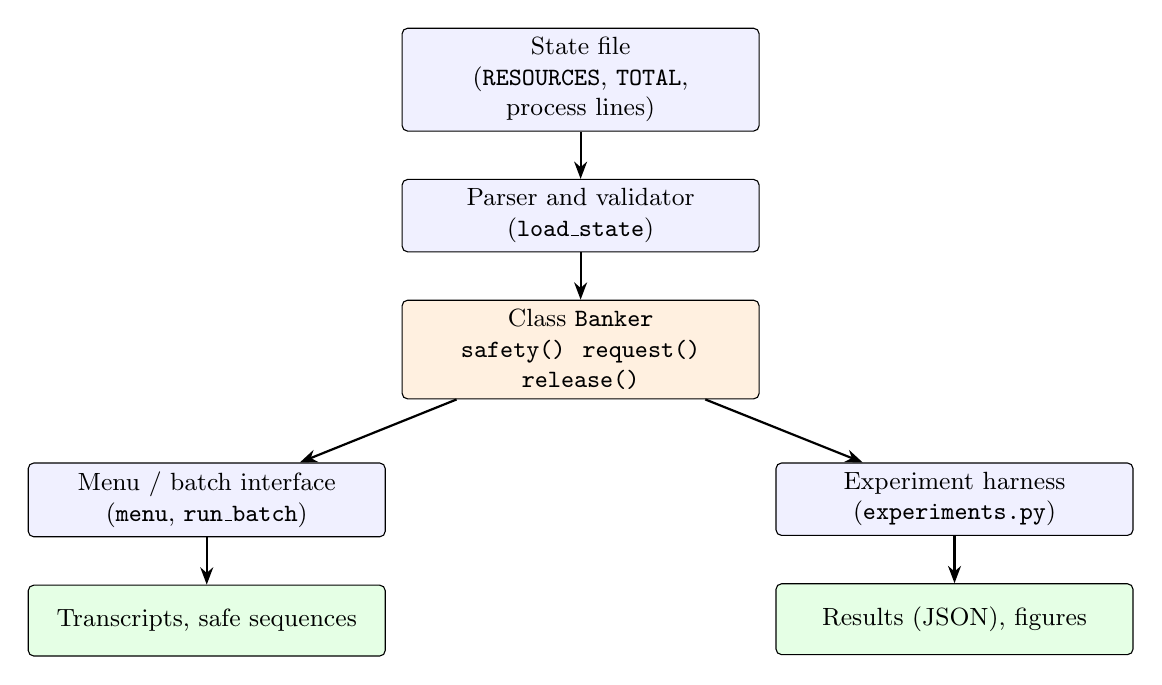
\begin{tikzpicture}[node distance=6mm and 10mm,
  blk/.style={rectangle,draw,rounded corners=2pt,minimum height=9mm,text width=4.3cm,align=center,font=\small,fill=blue!6}]
  \node[blk] (in) {State file\\ (\texttt{RESOURCES}, \texttt{TOTAL}, process lines)};
  \node[blk,below=of in] (par) {Parser and validator\\ (\texttt{load\_state})};
  \node[blk,below=of par,fill=orange!12] (core) {Class \texttt{Banker}\\ \texttt{safety()} \ \texttt{request()} \ \texttt{release()}};
  \node[blk,below left=8mm and 2mm of core] (ui) {Menu / batch interface\\ (\texttt{menu}, \texttt{run\_batch})};
  \node[blk,below right=8mm and 2mm of core] (exp) {Experiment harness\\ (\texttt{experiments.py})};
  \node[blk,below=of ui,fill=green!10] (out) {Transcripts, safe sequences};
  \node[blk,below=of exp,fill=green!10] (res) {Results (JSON), figures};
  \draw[arr] (in)--(par); \draw[arr] (par)--(core);
  \draw[arr] (core)--(ui); \draw[arr] (core)--(exp);
  \draw[arr] (ui)--(out); \draw[arr] (exp)--(res);
\end{tikzpicture}
\caption{Architecture of the Banker's-algorithm simulator.}
\label{fig:arch}
\end{figure}

\subsection{Experimental Design}
\textbf{Workloads.} Each trial uses $n=6$ processes and $m=3$ resource types with 10 instances of each. The maximum claims are random integers; the \emph{claim ratio} $\rho$ is the expected sum of the claims divided by the number of installed instances, and is varied from 0.6 to 3.0. For $\rho<1$ the claims fit into the system on average; for $\rho>1$ the system is over-committed and a poor policy can deadlock.

\textbf{Process behaviour.} Each process works in $K=4$ steps of one round each. Before each step it requests part of its remaining need (the last step requests everything that is still missing), and it returns all its resources after the last step.

\textbf{Compared policies.}
\begin{itemize}
    \item \emph{No avoidance}: a request is granted whenever enough instances are free.
    \item \emph{Banker's algorithm}: a request is granted only if the state remains safe.
    \item \emph{Prevention (all-at-once)}: a process requests its whole maximum claim at the beginning and works without further requests; this removes the hold-and-wait condition [7].
\end{itemize}

\textbf{Metrics.} (i) Percentage of workloads that end in deadlock, (ii) mean number of rounds until all processes have finished (only for runs that did not deadlock), and (iii) mean number of requests that had to wait. Every policy is run on identical random workloads (same seeds), with 2{,}000 workloads for every value of $\rho$. A deadlock is declared when no process is running and every unfinished process is waiting for a final request that exceeds $\text{Available}$.

% =============================================================================
\section{Implementation, Testing and Validation}
% =============================================================================
\subsection{Environment and Usage}
The program \texttt{bankers.py} is written in Python 3.12 and was developed and tested on Linux. It uses only the Python standard library. A system is described by a text file; Listing~\ref{lst:state} shows the textbook example [1] used throughout the report ($n=5$ processes, resource types $A$, $B$, $C$ with 10, 5 and 7 instances).

\begin{lstlisting}[style=term,caption={State file \texttt{textbook.txt}.},label={lst:state}]
RESOURCES A B C
TOTAL 10 5 7
P0  0 1 0 | 7 5 3        # process  allocation | maximum claim
P1  2 0 0 | 3 2 2
P2  3 0 2 | 9 0 2
P3  2 1 1 | 2 2 2
P4  0 0 2 | 4 3 3
\end{lstlisting}

\begin{lstlisting}[style=term,caption={Ways of running the program.},label={lst:usage}]
python3 bankers.py textbook.txt                    # menu-driven session
python3 bankers.py textbook.txt --safety           # only the safety check
python3 bankers.py textbook.txt --batch requests.txt   # scripted commands
python3 test_bankers.py -v                         # 20 unit tests
python3 experiments.py data                        # validation and experiments
\end{lstlisting}

The complete source code is given in Appendix~A.

\subsection{Core Functions}
Listing~\ref{lst:safety} shows the safety algorithm. It works on a copy of the allocation matrix, so it can be used on a ``pretend'' state without changing the real one, and it counts the \texttt{Need}$\le$\texttt{Work} comparisons for the complexity analysis.

\begin{lstlisting}[style=py,caption={Safety algorithm (method \texttt{Banker.safety}).},label={lst:safety}]
def safety(self, alloc=None):
    alloc = self.alloc if alloc is None else alloc
    n, m = self.n, self.m
    need = [[self.max[i][j] - alloc[i][j] for j in range(m)] for i in range(n)]
    work = [self.total[j] - sum(alloc[i][j] for i in range(n)) for j in range(m)]
    finish = [not self.active[i] for i in range(n)]
    seq, trace, checks = [], [], 0
    progress = True
    while progress:
        progress = False
        for i in range(n):
            if finish[i]:
                continue
            checks += 1
            if all(need[i][j] <= work[j] for j in range(m)):
                before = list(work)
                work = [work[j] + alloc[i][j] for j in range(m)]
                finish[i] = True
                seq.append(self.procs[i])
                trace.append((self.procs[i], before, list(need[i]), list(work)))
                progress = True
    return all(finish), seq, trace, checks
\end{lstlisting}

Listing~\ref{lst:request} shows the request algorithm. The pretend allocation is made on a copy (\texttt{trial}); the real matrix is replaced only after the safety test succeeds, so a denied request leaves the state unchanged.

\begin{lstlisting}[style=py,caption={Resource-request algorithm (method \texttt{Banker.request}).},label={lst:request}]
def request(self, pname, req):
    ...                                   # unknown / finished process, bad vector -> ERROR
    need, avail = self.need[i], self.available
    if any(req[j] > need[j] for j in range(self.m)):      # step 1
        return "ERROR", "... exceeds its maximum claim ..."
    if any(req[j] > avail[j] for j in range(self.m)):     # step 2
        return "WAIT", "Resources not available now ..."
    trial = [list(r) for r in self.alloc]                 # step 3: pretend allocation
    for j in range(self.m):
        trial[i][j] += req[j]
    safe, seq, _, _ = self.safety(trial)
    if not safe:                                          # step 4: roll back
        return "UNSAFE", "... would lead to an UNSAFE state. Request denied ..."
    self.alloc = trial                                    # commit
    return "GRANTED", "... New state is safe, safe sequence: <...>"
\end{lstlisting}

\subsection{Test Plan and Unit Tests}
Twenty unit tests (file \texttt{test\_bankers.py}) cover normal operation, every error path and the rollback behaviour. All tests pass (\texttt{Ran 20 tests ... OK}). Table~\ref{tab:tests} lists them.

\begin{table}[h!]
\centering
\caption{Unit tests and results.}
\label{tab:tests}
\small
\renewcommand{\arraystretch}{1.15}
\begin{tabular}{|c|p{6.4cm}|p{5.6cm}|c|}
\hline
\textbf{No.} & \textbf{Test} & \textbf{Expected behaviour} & \textbf{Result} \\ \hline
1 & Textbook state (Listing~\ref{lst:state}) & Safe, sequence $\langle P_1,P_3,P_4,P_0,P_2\rangle$ & Pass \\ \hline
2 & State in which no process can finish & Unsafe, empty sequence & Pass \\ \hline
3 & $P_1$ requests $(1,0,2)$ & Granted; Available becomes $(2,3,0)$ & Pass \\ \hline
4 & $P_4$ requests $(3,3,0)$ after test 3 & Wait (more than available) & Pass \\ \hline
5 & $P_0$ requests $(0,2,0)$ after test 3 & Denied: unsafe state & Pass \\ \hline
6 & Request larger than the declared need & Error: claim exceeded & Pass \\ \hline
7 & Request by an unknown process & Error & Pass \\ \hline
8 & Request vector of wrong length or negative & Error & Pass \\ \hline
9 & Release of $P_3$ & Returns $(2,1,1)$; Available $(5,4,3)$ & Pass \\ \hline
10 & Request of test 5 after $P_1$ has finished & Granted & Pass \\ \hline
11 & Denied request leaves the allocation unchanged & Matrix identical before and after & Pass \\ \hline
12 & Maximum claim larger than total & Input rejected & Pass \\ \hline
13 & Allocation larger than maximum claim & Input rejected & Pass \\ \hline
14 & Sum of allocations larger than total & Input rejected & Pass \\ \hline
15 & Malformed line in the state file & Input rejected & Pass \\ \hline
16 & Single resource, 10 units (3, 2, 2 held) & Safe & Pass \\ \hline
17 & Single resource, 10 units (4, 2, 2 held) & Unsafe & Pass \\ \hline
18 & Extra unit requested in test 16 state & Denied: unsafe & Pass \\ \hline
19 & Zero request & Granted, state unchanged & Pass \\ \hline
20 & Request by a process that has finished & Error & Pass \\ \hline
\end{tabular}
\end{table}

\subsection{Validation of the Safety Decision by Exhaustive Search}
The safety algorithm is a greedy method. To confirm that it never misses a safe sequence, it was compared with a reference that tries \emph{all} $n!$ completion orders. 20{,}000 random states were generated ($2\le n\le 6$, $1\le m\le 3$, 3--9 instances per type, random allocations and claims). Table~\ref{tab:e1} shows that the two methods gave the same answer in every case.

\begin{table}[h!]
\centering
\caption{Safety algorithm versus exhaustive search over all execution orders.}
\label{tab:e1}
\renewcommand{\arraystretch}{1.2}
\begin{tabular}{|l|c|}
\hline
Random states tested & 20{,}000 \\ \hline
States that are safe (by exhaustive search) & 9{,}141 \\ \hline
States that are unsafe (by exhaustive search) & 10{,}859 \\ \hline
\textbf{Cases in which both methods agree} & \textbf{20{,}000 (100\%)} \\ \hline
\end{tabular}
\end{table}

% =============================================================================
\section{Results and Discussion}
\label{sec:results}
% =============================================================================
All outputs below are the real, unedited output of \texttt{bankers.py} and \texttt{experiments.py}.

\subsection{Safety Check of the Textbook State}
Listing~\ref{lst:out-safety} shows the safety algorithm on the state of Listing~\ref{lst:state}. The initial free pool is $\text{Available}=(3,3,2)$. $P_1$ is the first process whose need $(1,2,2)$ fits into $\text{Work}$; after it finishes, $\text{Work}$ grows to $(5,3,2)$ and the next process can run, and so on. The system is safe with the safe sequence $\langle P_1,P_3,P_4,P_0,P_2\rangle$, and at the end $\text{Work}=(10,5,7)$, which equals $\text{Total}$: all instances have been returned. Figure~\ref{fig:work} shows how the free pool grows along the sequence.

\lstinputlisting[style=term,caption={Safety algorithm on the textbook state.},label={lst:out-safety}]{data/out_safety.txt}

\begin{figure}[h!]
\centering
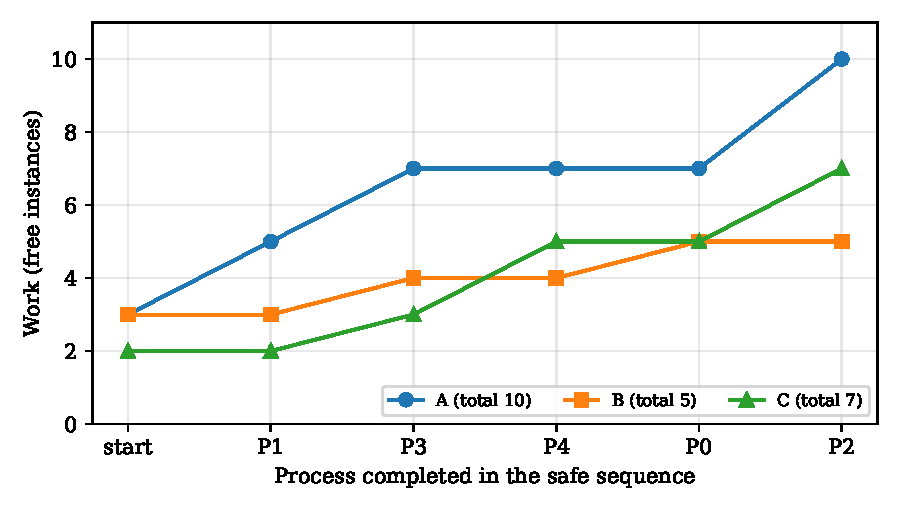
\includegraphics[width=0.78\linewidth]{figs/work_vector.pdf}
\caption{Free instances ($\text{Work}$) of each resource type along the safe sequence $\langle P_1,P_3,P_4,P_0,P_2\rangle$. Each completion returns the allocation of the finished process; at the end the free pool equals $\text{Total}=(10,5,7)$.}
\label{fig:work}
\end{figure}

\subsection{Handling of Resource Requests}
Listing~\ref{lst:out-req} shows a batch session on the same state. The first request, $P_1$ asking for $(1,0,2)$, is available and safe, so it is granted. Then $P_4$ asks for $(3,3,0)$: only $(2,3,0)$ is free, so $P_4$ must wait. The third request is the most interesting one: $P_0$ asks for $(0,2,0)$. The resources are free, but granting them would leave $\text{Available}=(2,1,0)$ and no process could be completed; the request is therefore \textbf{denied although it is available}, and the allocation is rolled back. The fourth request exceeds the declared claim and is reported as an error. After $P_1$ obtains its last $(0,2,0)$ and finishes, the same request of $P_0$ is granted, because the freed instances restore a safe sequence.

\lstinputlisting[style=term,caption={Batch session: grant, wait, unsafe denial, error and later grant.},label={lst:out-req}]{data/out_requests.txt}

\subsection{Unsafe State and Menu-Driven Session}
Listing~\ref{lst:out-unsafe} shows a state in which three processes each hold some resources and each still needs two more instances of both types, but nothing is free. No process can finish, so the state is unsafe; the program reports the blocked processes and returns exit code 2.

\lstinputlisting[style=term,caption={Detection of an unsafe state.},label={lst:out-unsafe}]{data/out_unsafe.txt}

Listing~\ref{lst:out-menu} shows the menu-driven mode. In the original state a request of $P_4$ for $(3,3,0)$ is refused as unsafe even though the resources are free, whereas after the grant to $P_1$ the same request waits for lack of resources (Listing~\ref{lst:out-req}): the reason for a refusal depends on the current state, and the program names it. Invalid input is reported without stopping the program.

\lstinputlisting[style=term,caption={Menu-driven session (excerpt after the first state display).},label={lst:out-menu}]{data/out_menu_trim.txt}

\subsection{Comparison of Policies on Random Workloads}
Table~\ref{tab:e2} and Figures~\ref{fig:deadlock}--\ref{fig:time} summarise the experiment described in Section~\ref{sec:method}: 2{,}000 random workloads for each of the eight claim ratios, 16{,}000 workloads per policy, identical workloads for all policies.

\begin{table}[h!]
\centering
\caption{Comparison of the three policies ($n=6$, $m=3$, 10 instances per type, 2{,}000 workloads per row). $^*$Mean rounds for ``None'' count only the runs that did not deadlock. ``Waits'' are requests that had to be repeated.}
\label{tab:e2}
\small
\renewcommand{\arraystretch}{1.15}
\begin{tabular}{|c|ccc|ccc|cc|}
\hline
 & \multicolumn{3}{c|}{\textbf{Deadlock (\%)}} & \multicolumn{3}{c|}{\textbf{Mean rounds to finish}} & \multicolumn{2}{c|}{\textbf{Mean waits}} \\
$\rho$ & None & Banker & Prev. & None$^*$ & Banker & Prev. & Banker & Prev. \\ \hline
0.6 & 0.0 & 0.0 & 0.0 & 4.0 & 4.0 & 4.1 & 0.0 & 0.1 \\
0.8 & 0.1 & 0.0 & 0.0 & 4.7 & 4.7 & 6.7 & 1.3 & 3.4 \\
1.0 & 0.2 & 0.0 & 0.0 & 4.7 & 4.7 & 6.7 & 1.4 & 3.5 \\
1.2 & 7.1 & 0.0 & 0.0 & 5.6 & 5.6 & 8.1 & 4.5 & 7.9 \\
1.5 & 36.8 & 0.0 & 0.0 & 6.4 & 6.8 & 9.6 & 8.7 & 12.6 \\
2.0 & 87.5 & 0.0 & 0.0 & 7.6 & 9.2 & 14.1 & 15.9 & 24.2 \\
2.5 & 95.3 & 0.0 & 0.0 & 7.9 & 10.3 & 16.4 & 19.1 & 31.3 \\
3.0 & 99.5 & 0.0 & 0.0 & 8.3 & 12.6 & 19.8 & 24.3 & 43.7 \\
\hline
\end{tabular}

\end{table}

\begin{figure}[h!]
\centering
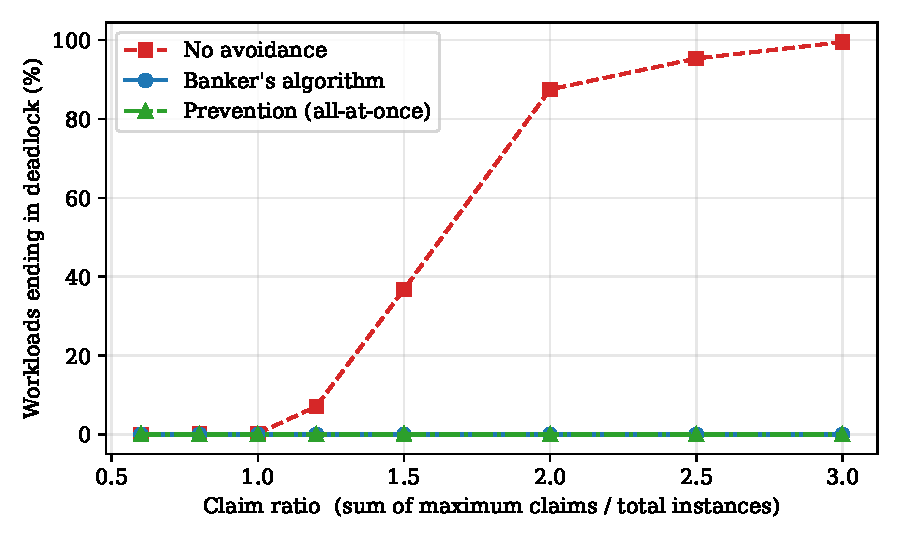
\includegraphics[width=0.82\linewidth]{figs/deadlock_rate.pdf}
\caption{Percentage of workloads that end in deadlock.}
\label{fig:deadlock}
\end{figure}

\begin{figure}[h!]
\centering
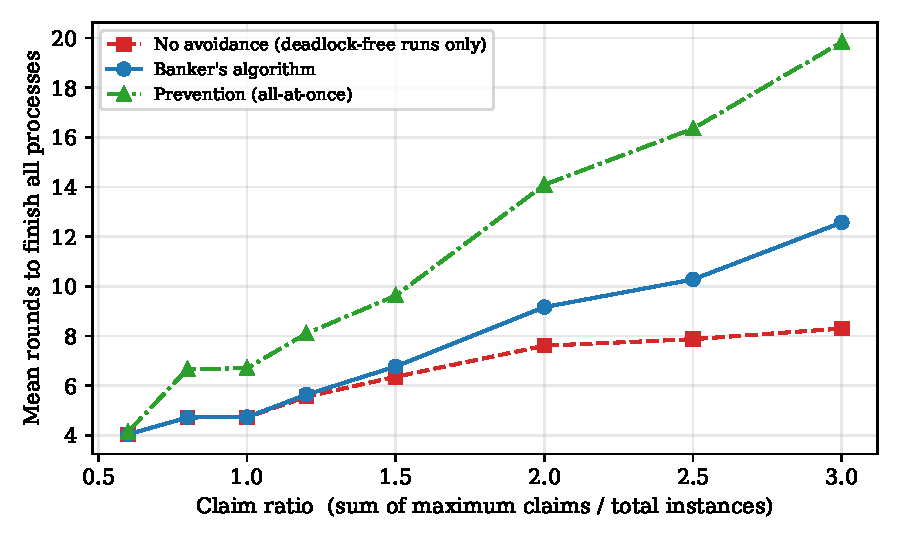
\includegraphics[width=0.82\linewidth]{figs/completion_time.pdf}
\caption{Mean number of rounds needed to finish all processes.}
\label{fig:time}
\end{figure}

\textbf{Deadlock.} Without avoidance the deadlock rate rises quickly once the system is over-committed: 7.1\% at $\rho=1.2$, 36.8\% at $\rho=1.5$, 87.5\% at $\rho=2.0$ and 99.5\% at $\rho=3.0$. Even at $\rho\le1$ a few workloads deadlock (0.1--0.2\%), because $\rho$ is an average over the three resource types and the claims for one type can still exceed what is installed. The Banker's algorithm and the prevention policy produced \textbf{no deadlock in any of the 16{,}000 workloads}, which agrees with the Theorem of Section~\ref{sec:method}. No run of any policy reached the round limit, so no starvation was observed in these experiments (Lemma~3).

\textbf{Completion time.} The ``no avoidance'' policy appears fastest, but only because its deadlocked runs, which never finish, are left out of the average. Among the two policies that always finish, the Banker's algorithm is clearly faster than all-at-once prevention from $\rho=0.8$ upward: it needs about 30--37\% fewer rounds (for example 12.6 versus 19.8 rounds at $\rho=3.0$, and 9.2 versus 14.1 at $\rho=2.0$). The reason is that prevention makes a process wait until its \emph{entire} claim is free and then locks all of it for the whole run, whereas the Banker's algorithm lets processes proceed step by step and delays only the requests that are really unsafe. For $\rho=0.6$ both policies need about four rounds because there is almost no competition.

\textbf{Effect of the number of processes.} Table~\ref{tab:e2n} repeats the experiment at $\rho=1.5$ with a different number of processes (1{,}500 workloads for each value). When the same total demand is divided among more processes, the claim of each process becomes smaller and deadlocks become rarer without avoidance, but the Banker's algorithm remains at 0\% for every $n$.

\begin{table}[h!]
\centering
\caption{Deadlock rate at $\rho=1.5$ for different numbers of processes.}
\label{tab:e2n}
\renewcommand{\arraystretch}{1.15}
\begin{tabular}{|c|c|c|}
\hline
\textbf{Processes $n$} & \textbf{No avoidance (\%)} & \textbf{Banker (\%)} \\ \hline
2 & 77.5 & 0.0 \\
3 & 76.5 & 0.0 \\
4 & 71.7 & 0.0 \\
6 & 33.9 & 0.0 \\
8 & 22.5 & 0.0 \\
10 & 7.1 & 0.0 \\
12 & 0.1 & 0.0 \\
\hline
\end{tabular}

\end{table}

\subsection{Cost of the Safety Algorithm}
The cost was measured on a worst-case state in which, in each pass, only the last unfinished process can run ($m=4$). Table~\ref{tab:e3} and Figure~\ref{fig:complexity} show that the number of $\text{Need}\le\text{Work}$ comparisons equals exactly $n(n+1)/2$ for every $n$, which confirms the quadratic bound of Section~\ref{sec:method}. The measured time grows by a factor of about 51 when $n$ grows from 100 to 800 (a factor of 64 would be exactly quadratic). The absolute times (milliseconds for hundreds of processes, in an interpreted language) depend on the computer and are meaningful only in relation to each other; for the small process counts of a real resource manager the test is cheap, but it must be repeated at every request.

\begin{table}[h!]
\centering
\caption{Worst-case cost of one safety check ($m=4$).}
\label{tab:e3}
\renewcommand{\arraystretch}{1.15}
\begin{tabular}{|c|c|c|c|}
\hline
\textbf{$n$} & \textbf{Measured comparisons} & \textbf{$n(n+1)/2$} & \textbf{Time per safety check (ms)} \\ \hline
10 & 55 & 55 & 0.10 \\
20 & 210 & 210 & 0.24 \\
50 & 1{,}275 & 1{,}275 & 1.18 \\
100 & 5{,}050 & 5{,}050 & 4.44 \\
200 & 20{,}100 & 20{,}100 & 17.36 \\
400 & 80{,}200 & 80{,}200 & 44.69 \\
800 & 320{,}400 & 320{,}400 & 227.37 \\
\hline
\end{tabular}

\end{table}

\begin{figure}[h!]
\centering
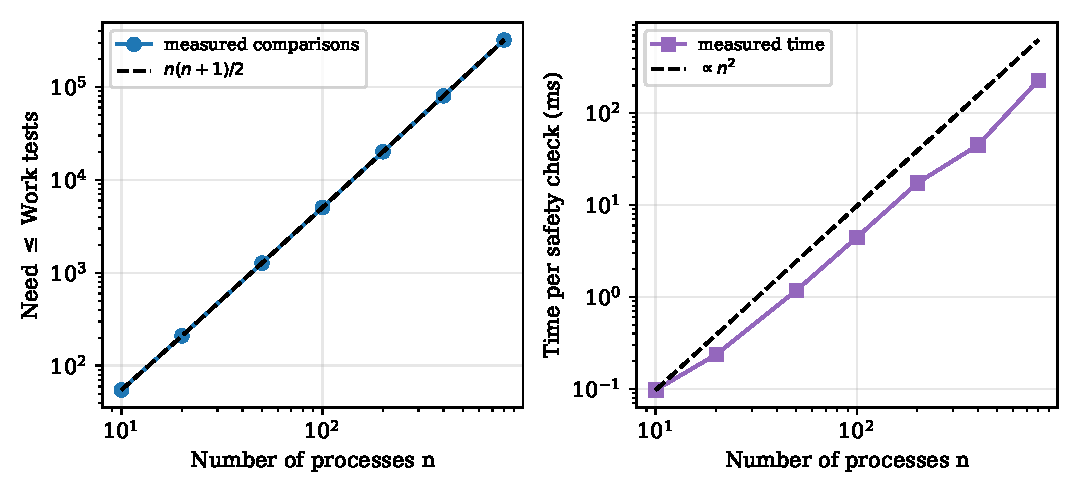
\includegraphics[width=0.95\linewidth]{figs/complexity.pdf}
\caption{Number of comparisons and running time of the safety algorithm against the number of processes (log--log scale).}
\label{fig:complexity}
\end{figure}

\subsection{Discussion and Limitations}
\begin{itemize}
    \item The results confirm the theory: avoidance guarantees deadlock freedom, and it does so at a lower cost in completion time than a simple prevention scheme, but with extra computation per request.
    \item The algorithm is \emph{conservative}: it denied available resources whenever safety could not be shown (Listing~\ref{lst:out-req}). Overstated claims therefore reduce its benefit.
    \item It requires the maximum claims in advance and a fixed set of processes and resources, which limits its use in general-purpose systems [1].
    \item It prevents deadlock but not starvation: a process whose requests are repeatedly unsafe may wait for a long time. The experiments did not show this, but the algorithm gives no guarantee.
    \item The experimental workloads are synthetic (uniform random claims, four steps per process, one request per round). The numbers show trends and should not be read as predictions for a particular real system.
    \item The simulator runs one request at a time; a real kernel would need locking around the shared tables.
\end{itemize}

% =============================================================================
\section{Sustainability and Societal Integration}
% =============================================================================
\subsection{Safe Resource Utilization}
The sustainability aspect of this project is \emph{safe resource utilization}: shared resources should be used so that the work already done is not lost and the system stays available. Deadlock recovery usually ends by terminating or rolling back processes [1], and the computation that was already performed is wasted. Avoidance removes this waste by refusing the one request that would lead to an unsafe state, and the process simply waits. In the experiments, the Banker's algorithm finished every workload without any forced termination, whereas the unprotected system left up to 99.5\% of the over-committed workloads stuck.

\subsection{Relevance to SDG 9 and SDG 16}
\begin{itemize}
    \item \textbf{SDG 9 (Industry, Innovation and Infrastructure):} Target 9.1 asks for reliable and resilient infrastructure. Operating systems, databases and cloud platforms form the digital infrastructure of industry; a resource manager that cannot deadlock increases its reliability. The project also builds the skills needed to design such infrastructure.
    \item \textbf{SDG 16 (Peace, Justice and Strong Institutions):} Target 16.6 asks for effective, accountable and transparent institutions. Public services that run on shared computing systems (for example payments, records and e-governance portals) must remain available and behave predictably. The simulator also illustrates transparency: every decision is explained (granted, wait, unsafe, or error), so a denied request can be audited.
\end{itemize}

\subsection{Impact on Society, Environment and Ethics}
\begin{itemize}
    \item \textbf{Social:} fewer service freezes mean more dependable digital services; the open, readable code and the explanatory output support education.
    \item \textbf{Environmental:} avoiding repeated restarts and re-computation reduces the processor time spent on lost work. The effect was not measured in this project, so no figure is claimed.
    \item \textbf{Fairness and ethics:} because the algorithm can postpone a request indefinitely, fairness must be considered when it is used with priorities; claims must be stated honestly because exaggerated claims waste capacity of other users.
    \item \textbf{Cost:} the method needs no special hardware; its cost is the extra computation of the safety test, quantified in Section~\ref{sec:results}.
\end{itemize}

% =============================================================================
\section{Conclusion and Future Work}
% =============================================================================
\subsection{Conclusion}
This project implemented the Banker's algorithm as a transparent, tested simulator that reads allocation and maximum-claim data, finds safe sequences and decides whether each resource request is granted, delayed or denied. The theoretical analysis shows that granting only checked requests keeps the system in a safe state and therefore deadlock-free. The implementation agreed with an exhaustive search on 20{,}000 random states and passed 20 unit tests. In 16{,}000 random workloads per policy, the Banker's algorithm never deadlocked, while the unprotected system deadlocked in up to 99.5\% of the over-committed workloads; compared with all-at-once prevention, it needed about 30--37\% fewer rounds. The price is a safety test of cost $O(mn^2)$ at every request, which was confirmed by measurement, and the need to know maximum claims in advance. The project thus gives a complete, evidence-based answer to the problem statement and meets the expected outcome of applying a deadlock-avoidance method to resource allocation.

\subsection{Future Work}
\begin{itemize}
    \item Implement the faster variants of the algorithm [9] and compare their measured cost.
    \item Add a deadlock-\emph{detection} algorithm and compare avoidance, prevention and detection-with-recovery in the same experiment.
    \item Support processes that arrive and leave at run time and dynamic changes of the resource pool.
    \item Add an ageing rule to guarantee that a process cannot be postponed indefinitely.
    \item Use real traces of lock or resource usage instead of synthetic workloads, and provide a graphical front end for teaching.
\end{itemize}

% ------------------ Mapping of POs and SDGs ------------------
\clearpage
\phantomsection
\addcontentsline{toc}{chapter}{Mapping of Program Outcomes (POs) and Sustainable Development Goals (SDGs)}
\chapter*{Mapping of Program Outcomes (POs) and Sustainable Development Goals (SDGs)}

\noindent\textbf{1. Contribution to Program Outcomes (POs)}

The project contributes to the following Program Outcomes:

\bigskip
\noindent\textbf{PO1: Engineering Knowledge (WP1) : Apply knowledge of mathematics, natural science, computing, engineering fundamentals and an engineering specialization as specified in WK1 to WK4 respectively to develop to the solution of complex engineering problems}\\
The project applies operating-system theory (resources, processes, the necessary conditions of deadlock), discrete mathematics (vector inequalities, safe-state definition, induction proofs) and algorithm analysis ($O(mn^2)$ complexity) to design and justify a deadlock-avoidance method.

\bigskip
\noindent\textbf{PO2: Problem Analysis (WP7): Identify, formulate, review research literature and analyze complex engineering problems reaching substantiated conclusions with consideration for sustainable development. (WK1 to WK4)}\\
The deadlock problem was formulated precisely (Section 2), alternative solutions were reviewed in the literature (Sections 3 and 4), and conclusions were substantiated by proofs, an exhaustive-search check and Monte-Carlo experiments, with attention to the avoidance of wasted work.

\bigskip
\noindent\textbf{PO3: Design/Development of Solutions (WP7): Design creative solutions for complex engineering problems and design/develop systems/components/processes to meet identified needs with consideration for the public health and safety, whole-life cost, net zero carbon, culture, society and environment as required. (WK5)}\\
A modular simulator (parser, algorithm class, menu and batch interfaces, experiment harness) was designed and built. Its explanatory messages and input validation make the system safe and understandable to use, and the method needs no special hardware.

\bigskip
\noindent\textbf{PO4: Conduct Investigations of Complex Problem (WP4) : Conduct investigations of complex engineering problems using research-based knowledge including design of experiments, modelling, analysis \& interpretation of data to provide valid conclusions. (WK8)}\\
The project designed controlled experiments (identical random workloads for all policies, fixed seeds, 16{,}000 workloads per policy), modelled process behaviour, and interpreted deadlock rates, completion times and algorithm cost to draw valid conclusions.

\bigskip
\noindent\textbf{PO5: Engineering Tool  (WP5): Create, select and apply appropriate techniques, resources and modern engineering \& IT tools, including prediction and modelling recognizing their limitations to solve complex engineering problems. (WK2 and WK6)}\\
Python 3, the unittest framework, Matplotlib and \LaTeX{} were used to implement, test, analyse and document the work. The limitations of the synthetic workload model are stated in Section 7.6.

\bigskip
\noindent\textbf{PO6: The Engineer and The World: Analyze and evaluate societal and environmental aspects while solving complex engineering problems for its impact on sustainability with reference to economy, health, safety, legal framework, culture and environment. (WK1, WK5, and WK7)}\\
Section 8 evaluates the societal and environmental aspects of safe resource utilization: reliable digital services, less wasted computation, fairness of allocation and the cost of the safety test.

\bigskip
\noindent\textbf{PO7: Ethics (WP7): Apply ethical principles and commit to professional ethics, human values, diversity and inclusion; adhere to national \& international laws. (WK9)}\\
Results are reported honestly, including the limits of the method (conservative denials, no starvation guarantee, synthetic workloads); sources are acknowledged in the references and the work is the team's own implementation.

\bigskip
\noindent\textbf{PO8: Individual and Collaborative Team work (WP6): Function effectively as an individual, and as a member or leader in diverse/multi-disciplinary teams.}\\
The work (analysis, implementation, testing, experiments and report) was carried out by a team of three students of Batch No.~1, integrating the parts into one tested program and one report.

\bigskip
\noindent\textbf{PO9: Communication (WP7): Communicate effectively and inclusively within the engineering community and society at large, such as being able to comprehend and write effective reports and design documentation, make effective presentations considering cultural, language, and learning differences}\\
A structured technical report with flowcharts, tables, graphs, annotated transcripts and fully commented source code was prepared; the program itself explains each decision in plain language.

\bigskip
\noindent\textbf{PO10: Project Management and Finance (WP2): Apply knowledge and understanding of engineering management principles and economic decision-making and apply these to one's own work, as a member and leader in a team, and to manage projects and in multidisciplinary environments}\\
The two-week project was divided into analysis, design, implementation, testing, experiments and documentation, and the trade-off between safety and run-time cost was evaluated as an economic decision (Sections 3.2 and 7.5).

\bigskip
\noindent\textbf{PO11: Life-Long Learning (WP3): Recognize the need for, and have the preparation and ability for i) independent and life-long learning ii) adaptability to new and emerging technologies and iii) critical thinking in the broadest context of technological change. (WK8)}\\
The team studied the original literature on deadlock, learned to design reproducible experiments and to prove properties of an algorithm, and identified future directions (faster variants, detection, dynamic systems) for further independent learning.

\bigskip
\noindent\textbf{2. Alignment with Sustainable Development Goals (SDGs)}

The project is aligned with the following SDGs:

\bigskip
\noindent\textbf{SDG 9: Industry, Innovation and Infrastructure}\\
Contributes to reliable and resilient digital infrastructure by showing how shared resources can be allocated without deadlock (Target 9.1) and by building related engineering skills.

\bigskip
\noindent\textbf{SDG 16: Peace, Justice and Strong Institutions}\\
Supports effective, accountable and transparent institutions (Target 16.6) by promoting dependable computing services whose allocation decisions are explainable and auditable.

\begin{thebibliography}{99}
\bibitem{silb} A. Silberschatz, P. B. Galvin and G. Gagne, \textit{Operating System Concepts}, 10th ed., Wiley, 2018.
\bibitem{tan} A. S. Tanenbaum and H. Bos, \textit{Modern Operating Systems}, 4th ed., Pearson, 2015.
\bibitem{stal} W. Stallings, \textit{Operating Systems: Internals and Design Principles}, 9th ed., Pearson, 2018.
\bibitem{dij} E. W. Dijkstra, ``Cooperating sequential processes,'' Technical Report EWD-123, Technological University Eindhoven, The Netherlands, 1965.
\bibitem{hab} A. N. Habermann, ``Prevention of system deadlocks,'' \textit{Communications of the ACM}, vol. 12, no. 7, pp. 373--377, 385, July 1969.
\bibitem{cof} E. G. Coffman, M. J. Elphick and A. Shoshani, ``System deadlocks,'' \textit{ACM Computing Surveys}, vol. 3, no. 2, pp. 67--78, 1971.
\bibitem{hav} J. W. Havender, ``Avoiding deadlock in multitasking systems,'' \textit{IBM Systems Journal}, vol. 7, no. 2, pp. 74--84, 1968.
\bibitem{holt} R. C. Holt, ``Some deadlock properties of computer systems,'' \textit{ACM Computing Surveys}, vol. 4, no. 3, pp. 179--196, 1972.
\bibitem{bel} F. Belik, ``Deadlock avoidance with a modified banker's algorithm,'' \textit{BIT}, vol. 27, pp. 290--305, 1987. doi:10.1007/BF01933724.
\bibitem{sha} L. Sha, R. Rajkumar and J. P. Lehoczky, ``Priority inheritance protocols: an approach to real-time synchronization,'' \textit{IEEE Transactions on Computers}, vol. 39, no. 9, pp. 1175--1185, 1990.
\bibitem{posix} IEEE and The Open Group, \textit{IEEE Std 1003.1-2017 (POSIX.1-2017), Standard for Information Technology -- Portable Operating System Interface}, 2018.
\bibitem{iso} ISO/IEC 25010:2011, \textit{Systems and software engineering -- Systems and software Quality Requirements and Evaluation (SQuaRE) -- System and software quality models}, 2011.
\bibitem{sdg} United Nations, \textit{Transforming our world: the 2030 Agenda for Sustainable Development}, A/RES/70/1, 2015.
\end{thebibliography}

% ------------------ Appendix ------------------
\appendix
\chapter*{Appendix A: Source Code of \texttt{bankers.py}}
\addcontentsline{toc}{chapter}{Appendix A: Source Code of bankers.py}
\lstinputlisting[style=py]{code/bankers.py}

\chapter*{Appendix B: Input Files}
\addcontentsline{toc}{chapter}{Appendix B: Input Files}
\noindent\textbf{Request script} (\texttt{requests.txt}):
\lstinputlisting[style=term]{data/requests.txt}
\noindent\textbf{Unsafe state} (\texttt{unsafe.txt}):
\lstinputlisting[style=term]{data/unsafe.txt}
\noindent The experiment program (\texttt{experiments.py}), the unit tests (\texttt{test\_bankers.py}), the figure script and all raw results (\texttt{results.json}) are supplied with the source files of this report.

\end{document}
